\documentclass[a4paper,12pt]{article}
\usepackage{graphicx}
\usepackage{hyperref}
\usepackage{amsmath}
\usepackage{times}
\usepackage{xcolor}
\usepackage{amsfonts}
\usepackage{garamondx}
\usepackage{framed}  %This is to use the shaded environment


\textwidth=6.2in
\textheight=8.5in
%\parskip=.3cm
\oddsidemargin=.1in
\evensidemargin=.1in
\headheight=-.3in
\setlength{\parindent}{0pt}



% \renewcommand{\baselinestretch}{1} 
% \setlength{\parskip}{\baselineskip}
% \setlength{\parindent}{0pt}
% \setlength{\marginparwidth}{2.5cm}


\newcommand{\scscst}{\scriptscriptstyle}
\newcommand{\scst}{\scriptstyle}
\newcommand{\Robject}[1]{{\texttt{#1}}}
\newcommand{\Rfunction}[1]{{\texttt{#1}}}
\newcommand{\Rclass}[1]{\textit{#1}}
\newcommand{\Rpackage}[1]{\textit{#1}}
\newcommand{\Rexpression}[1]{\texttt{#1}}
\newcommand{\Rmethod}[1]{{\texttt{#1}}}
\newcommand{\Rfunarg}[1]{{\texttt{#1}}}

\newcommand\boldblue[1]{\textcolor{blue}{\textbf{#1}}}
\newcommand{\code}[1]{\texttt{#1}}

\usepackage{Sweave}
\begin{document}
\definecolor{shadecolor}{gray}{0.95} %this is defining the color of the background in the shaded environment

\Sconcordance{concordance:3_Course_Notes-knitr.tex:3_Course_Notes-knitr.Rnw:%
1 50 1 1 0 4 1 1 7 12 1 1 7 1 1 1 7 94 1 1 2 1 0 3 1 3 0 1 2 6 1 1 2 1 %
0 1 1 1 2 1 1 3 0 1 2 9 1 1 2 4 0 1 2 4 1 1 2 1 0 1 1 3 0 1 2 45 1 1 4 %
6 0 1 2 12 1 1 2 4 0 1 2 5 1}




%------------------------------------------------------------
\title{Using R as a Research Tool.}
%------------------------------------------------------------
\author{Susan Johnston: \href{mailto:Susan.Johnston@ed.ac.uk}{Susan.Johnston@ed.ac.uk}  \\ 
        Demonstrators: Gergana Dalaskova, John Godlee \\
        Hat-Tips: Kyle Dexter, Coding Club}
%\date{}









\maketitle

%\tableofcontents


%-------------------------------------------
\section {Introduction}
%--------------------------------------------

\subsection {What is \boldblue{R}?}

\boldblue{R} began its life in New Zealand in 1993 as a language and environment for statistical computing and graphics. It is an interpreted programming language, meaning that rather than pointing and clicking, the user instead types in commands. It is \textbf{free} and works across all platforms.


\subsection {Why use \boldblue{R}?}

\begin{center}
``\texttt{This is R. There is no if. Only how.}'' \\
\code{{-}{-} Simon `Yoda' Blomberg, R-help (April 2005)}

\end{center}


Almost anything is possible in \boldblue{R}. It is fast becoming the \textit{lingua franca} of academic research and data science. It is used for:

\begin{itemize}
\item Processing and tidying data 
\item Statistical analyses
\item Data visualistion (\code{ggplot})
\item Creating interactive web applications (\code{shiny})
\item Generating reports and presentations (\code{knitr}, \code{slidify})
\item Creating portable projects (RStudio Projects)
\end{itemize}

The analytical power of \boldblue{R} lies in its many packages (11,172 at the time of writing). At least 300 of these are written for ecologists and evolutionary biologists. A list of packages are hosted on the Comprehensive R Archive Network (known as \textbf{CRAN}): \url{https://cran.r-project.org/}.

\subsection {What we hope to achieve in this session.}

Before beginning this course, we asked you to complete the 


%-------------------------------------------
\section {Getting Started: R and the RStudio Environment.}
%--------------------------------------------

\subsection {Installing R and RStudio.}

R can be downloaded from the CRAN website. Whilst the CRAN download version provides a simple user interface, we recommend that R is run through the software RStudio. This is open-source, free, and available at \url{http://www.rstudio.com/}. [NB. It is important to install R first and RStudio second.]

\subsection {Using RStudio.}

Open a new R Script (\texttt{File > New File > R Script}) and save it. RStudio should look something like Figure \ref{fig:R_Studio}. 
\\


\begin{figure}[h]
	\centering 
	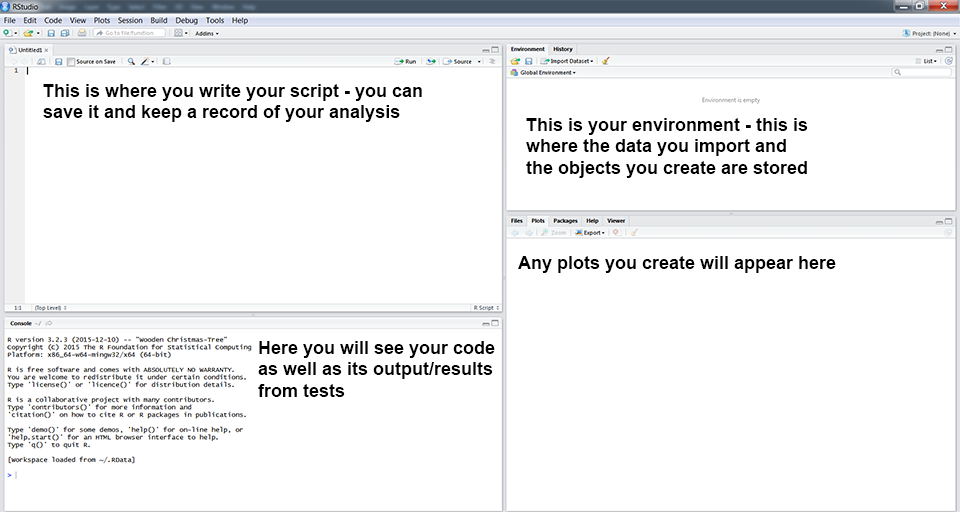
\includegraphics[width=1.1\textwidth]{figs/R_Studio.png}
	\caption{The RStudio Environment. Taken from OurCodingClub.io}
	\label{fig:R_Studio}
\end{figure} 

On the lower left is the \textit{Console} pane - this is the engine of R. You can give instructions to R by directly typing at the prompt (\texttt{>}). 
\\

On the upper left is your new R Script - here, you can write commands and send them to the console by clicking ``\texttt{Run}'' or by typing \texttt{Ctrl-Enter} (or \texttt{Cmd-Enter}). 
\\

On the lower right, you can browse the packages installed on your machine, open files and search R Help. This pane will also show plots when we run them later in the practical.
\\

\fbox{\begin{minipage}{36em}
\Large{\textbf{Exercise 1.}}

\normalsize
Try running some basic commands directly in the console and from the R Script:
\end{minipage}}


\begin{shaded}
\begin{Schunk}
\begin{Sinput}
> 2+3
\end{Sinput}
\begin{Soutput}
[1] 5
\end{Soutput}
\begin{Sinput}
> 1:10
\end{Sinput}
\begin{Soutput}
 [1]  1  2  3  4  5  6  7  8  9 10
\end{Soutput}
\begin{Sinput}
> seq(1, 20, 4)
\end{Sinput}
\begin{Soutput}
[1]  1  5  9 13 17
\end{Soutput}
\begin{Sinput}
> mean(c(3, 6, 9, 3, 6, 7))
\end{Sinput}
\begin{Soutput}
[1] 5.666667
\end{Soutput}
\end{Schunk}
\end{shaded}

\fbox{\begin{minipage}{36em}
Let's assign a sequence of numbers to an object, \texttt{x}:
\end{minipage}}

\begin{shaded}
\begin{Schunk}
\begin{Sinput}
> x <- 1:10
> x
\end{Sinput}
\begin{Soutput}
 [1]  1  2  3  4  5  6  7  8  9 10
\end{Soutput}
\begin{Sinput}
> y <- seq(0, 4.5, 0.5)
> y
\end{Sinput}
\begin{Soutput}
 [1] 0.0 0.5 1.0 1.5 2.0 2.5 3.0 3.5 4.0 4.5
\end{Soutput}
\end{Schunk}
\end{shaded}


You can see that in the upper right pane, we can see this new objects \texttt{x} and \texttt{y} in the environment.

\subsection {Finding Help with R.}

The fastest way to find help in R is to search using \texttt{?}. For example:

\begin{shaded}
\begin{Schunk}
\begin{Sinput}
> ?mean
\end{Sinput}
\end{Schunk}
\end{shaded}

should bring up a help page for the function \texttt{mean()} in the lower right corner. Typing two question marks: 

\begin{shaded}
\begin{Schunk}
\begin{Sinput}
> ??mean
> ??"standard error"
\end{Sinput}
\end{Schunk}
\end{shaded}

will search all help files and return a list of those that match. \\\\

\fbox{\begin{minipage}{36em}
\Large{\textbf{Exercise 2.}}

\normalsize
\begin{enumerate}
\item Using only \texttt{?} and/or \texttt{??}, find a function for calculating the standard deviation. What is the standard deviation of \texttt{x}?

\item Using \texttt{?}, find the help file for the \texttt{sort()} function. Sort \texttt{x} and \texttt{y} in reverse order.\\
\end{enumerate}
\end{minipage}}


\subsection {Troubleshooting and finding help outside of R.}

\begin{itemize}
\item Coding Club Tutorials \& Useful Links \url{https://ourcodingclub.github.io/}
\item Stack Overflow \url{https://stackoverflow.com/}: Try searching with the tag [R]
\item Google
\item RStudio Cheatsheets \url{https://www.rstudio.com/resources/cheatsheets/}
\end{itemize}


%-------------------------------------------
\section {Loading and Preparing Data.}
%--------------------------------------------



\end{document}
